%\documentclass[9pt]{book}
\documentclass[landscape,14pt]{oblivoir}
    \usepackage{a4wide}
    \usepackage{palatino}
    \usepackage{newcent}
    \usepackage{amsmath,amsfonts,amssymb}
	\usepackage{graphics} % for pdf, bitmapped graphics files
	\usepackage{epsfig} % for postscript graphics files
	\usepackage{xcolor}

    \setlength{\parindent}{0mm}
    \setlength{\textheight}{183.0mm}
    \setlength{\oddsidemargin}{-11.0mm}
    \setlength{\textwidth}{243.5mm}
   \setlength{\topmargin}{-30.0mm} 

\begin{document}

    \baselineskip 20pt
    \thispagestyle{empty}
    %!TEX root = ../main.tex
\setcounter{chapter}{7}
\setcounter{section}{0}
\section{Digitization}
\vspace{-8pt} \hrule \hrule \hrule \hrule \hrule  \vspace{12pt}
\begin{enumerate}
 \item Most control systems use digital computers (usually microprocessors) to implement the controller. 
 \item Sampler and A/D Converter, D/A Converter and ZOH (Zeroth-Order Holding), and Clock
 \item The computation of error signal $e(t)$ and the dynamic compensation $D_c(s)$ can all be accomplished in a digital computer. 
 \item Difference equation for discrete-time system $\leftrightarrow$ Differential equation for continuous-time system 
 \item Two basic techniques for finding the difference equations for the digital controller, from $D_c(s)$ to $D_d(z)$ 
 \begin{itemize}
  \item Discrete equivalent - section 8.3 
  \item Discrete design  - section 8.7 
 \end{itemize} 
 \item The analog output of the sensor is sampled and converted to a digital number in the analog-to-digital (A/D) converter. (Sampler and ADC)
 \begin{itemize}
  \item Conversion from the continuous analog signal $y(t)$ to the discrete digital samples $y(kT)$ occurs repeatedly at instants of time $T$ apart where $T$ is the sample period [$s$] and $1/T$ is the sample rate [$Hz$].
  \begin{align*}
   y(t) ~~~~ \rightarrow~~~~~y (k) = y(kT) ~~~~\mbox{with} ~~ t = kT  
  \end{align*}
  where $k$ is an integer and $T$ is a fixed value (sample period, or sampling time). 
  \item The sampled signal is $y(kT)$, where $k$ can take on any integer value. 
  \item It is often written simply as $y(k)$. We call this type of variable a discrete signal. 
 \end{itemize}  

\end{enumerate}

   
    \newpage
    %!TEX root = ../main.tex
\setcounter{chapter}{7}
\setcounter{section}{0}

%
\section{Digitization}
\vspace{-8pt} \hrule \hrule \hrule \hrule \hrule  \vspace{12pt}


\begin{enumerate}\addtocounter{enumi}{6}
 \item The D/A converter changes the digital binary number to an analog voltage, and a zeroth-order hold maintains the same voltage throughout the sample period $T$. (DAC and ZOH)

 \begin{itemize}
  \item Because each value of $u(kT)$ in Fig. 8.1(b) is held constant until the next value is available from the computer, the continuous value of $u(t)$ consists of steps (see Fig. 8.2) that, on average, are delayed from a fit to $u(kT)$ by $T/2$ as shown in the figure. 
  \item Sample rates should be at least 20 times the bandwidth in order to assure that the digital controller will match the performance of the continuous controller.
  \item If we simply incorporate this $T/2$ delay into a continuous analysis of the system, an excellent prediction results in, especially, for sample rates much slower than 20 times bandwidth.
 \end{itemize}
 \item A system having both discrete and continuous signals is called a `sampled data system'. 

\end{enumerate}

   
    \newpage
    %!TEX root = ../main.tex
\setcounter{chapter}{7}
\setcounter{section}{0}
\section{Digitization}
\vspace{-8pt} \hrule \hrule \hrule \hrule \hrule  \vspace{12pt}
\begin{figure}[!hb]
    \centering
    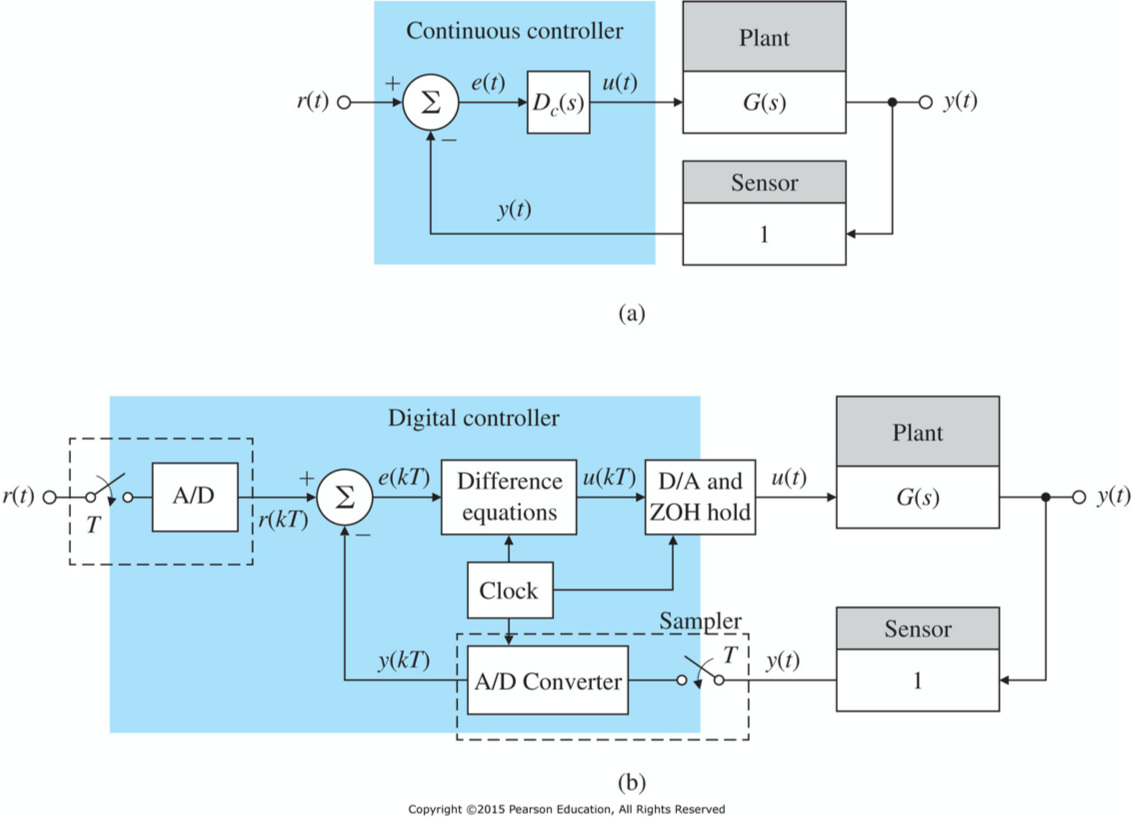
\includegraphics[width=20cm]{./FIG_Franklin/fig8-1.png}
\end{figure}   
    \newpage
    %!TEX root = ../main.tex
\setcounter{chapter}{7}
\setcounter{section}{0}
\section{Digitization}
\vspace{-8pt} \hrule \hrule \hrule \hrule \hrule  \vspace{12pt}
 \begin{itemize}
  \item Continuous-time signal: Both domain and range are continuous, $y(t)$

  \item Discrete-time signal: Domain is discrete and range is continuous, $y(k)$ or $y(kT)$

  \item Digital signal: Both domain and range are discrete, $y_d(k)$
    \begin{figure}[!hb]
        \centering
        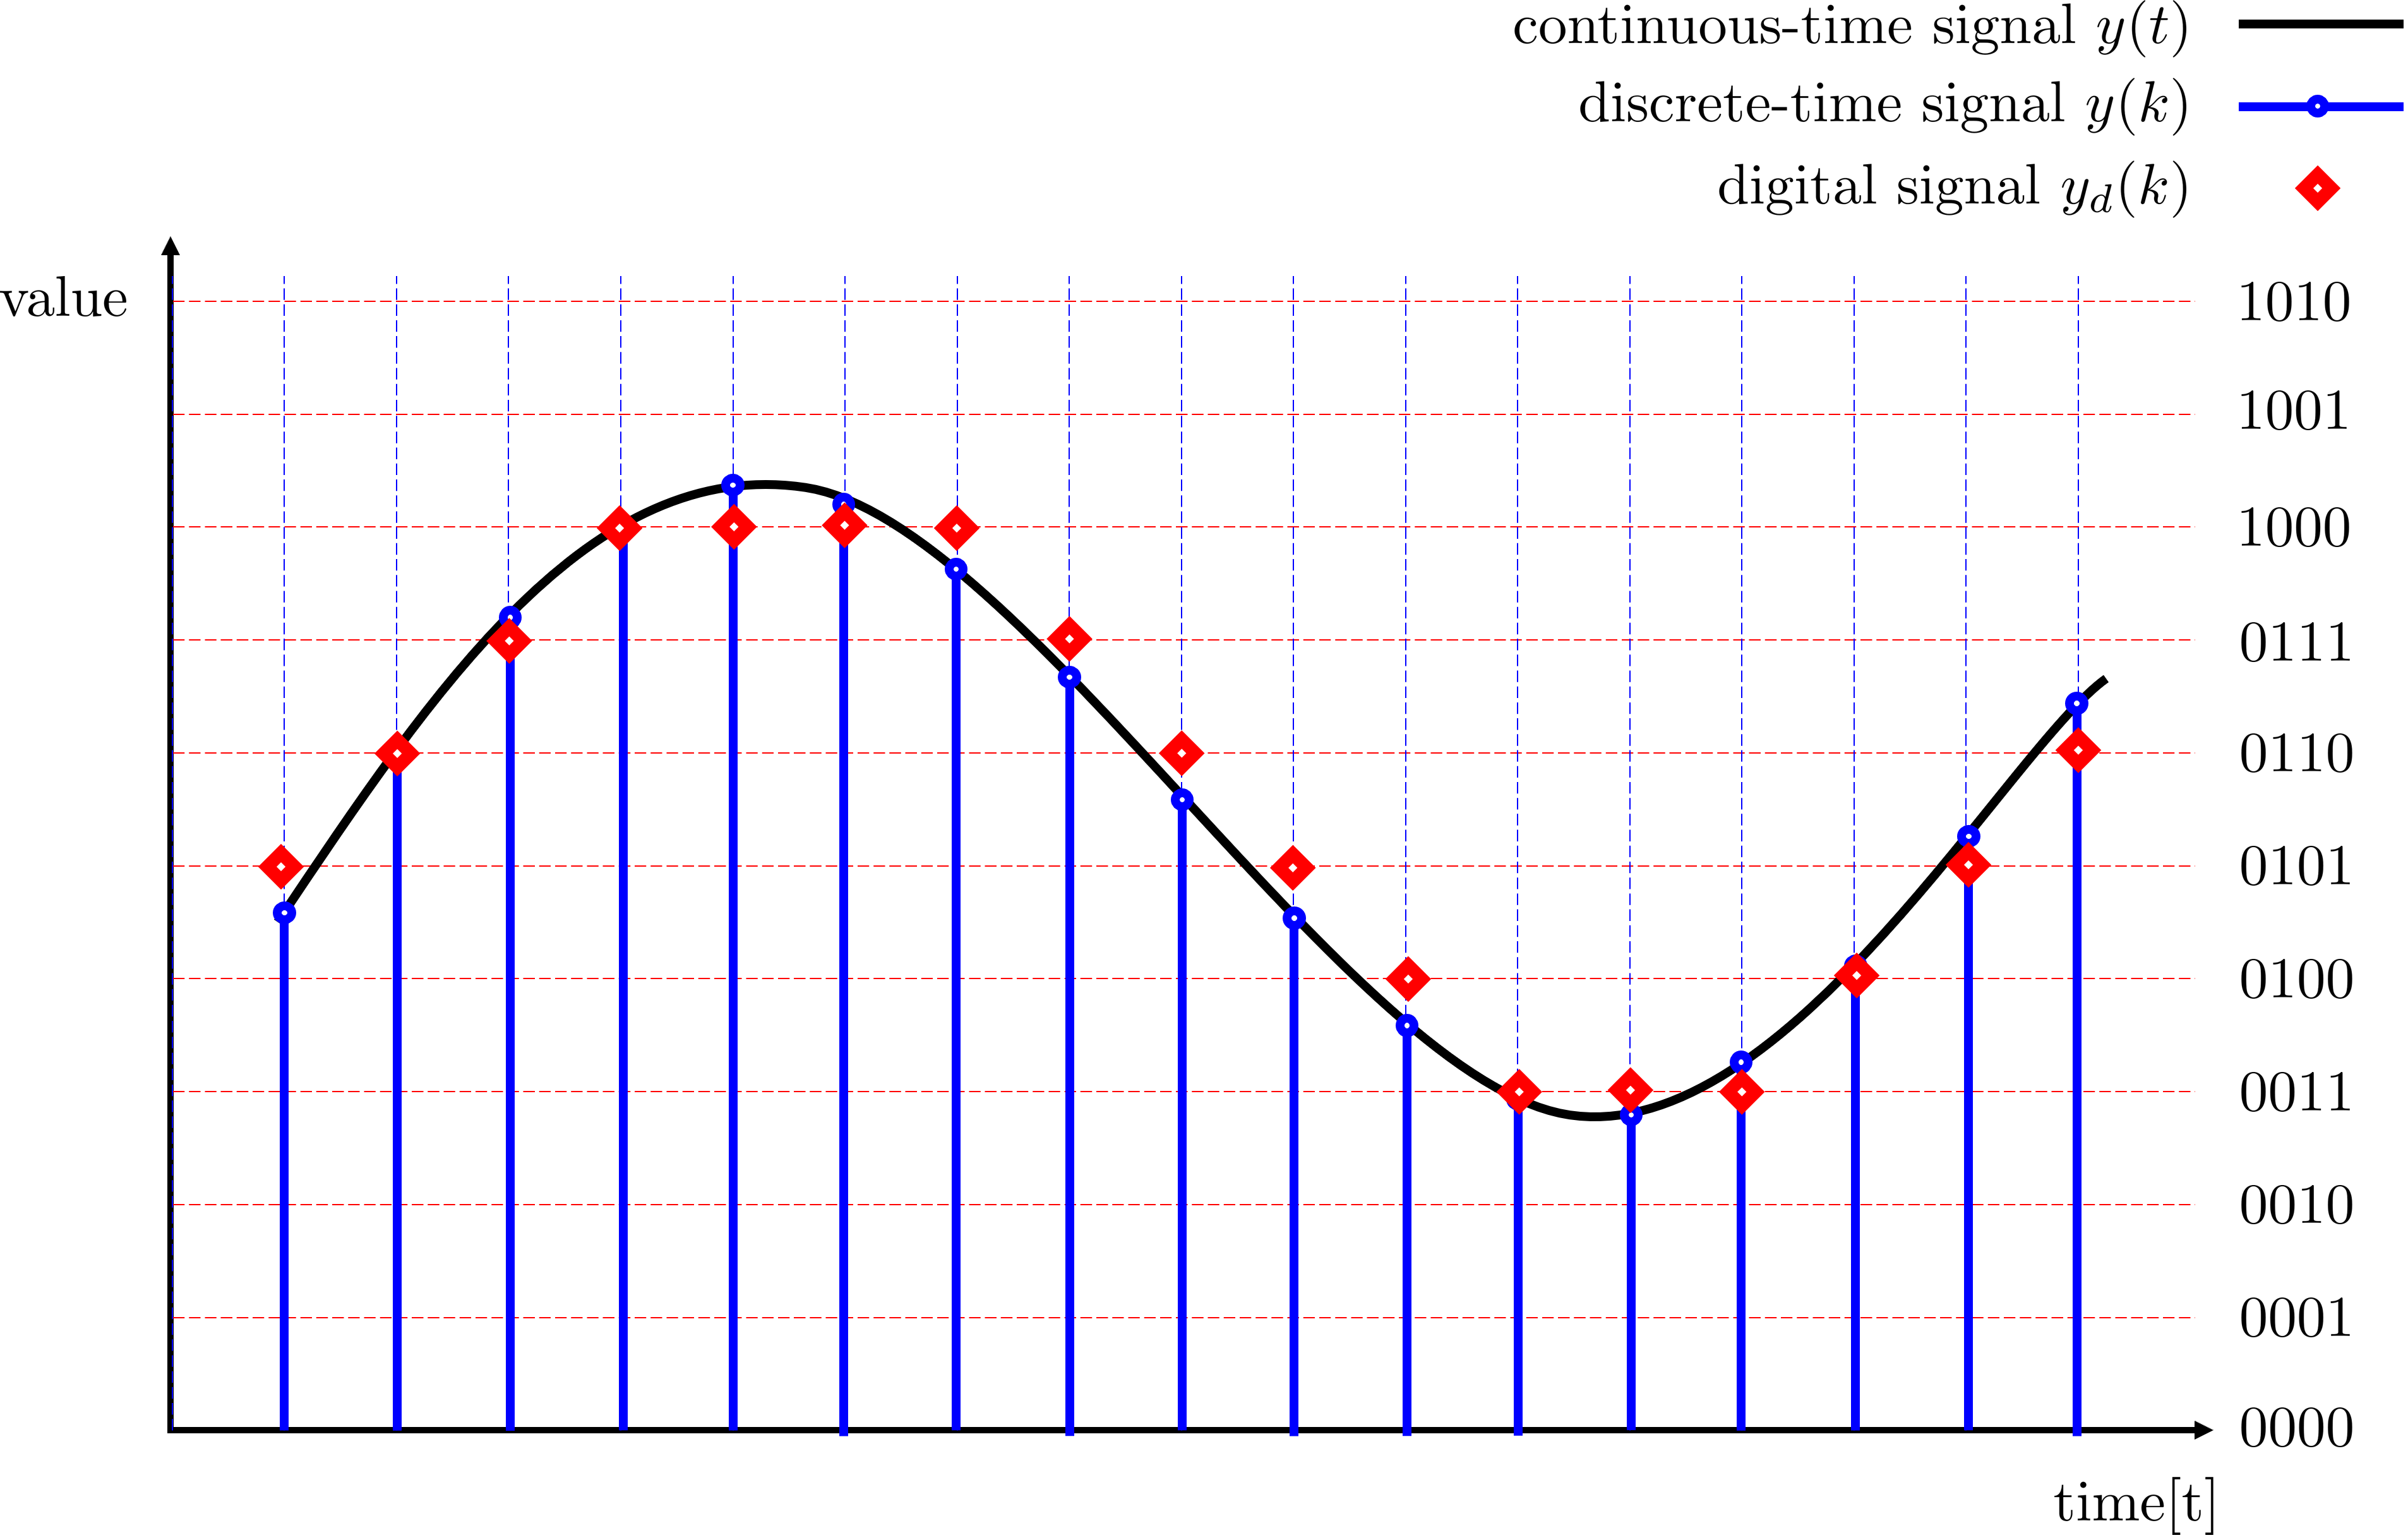
\includegraphics[width=20cm]{./FIG_Franklin/fig8-smc1.png}
    \end{figure}
 \end{itemize}    
    \newpage
    %!TEX root = ../main.tex
\setcounter{chapter}{7}
\setcounter{section}{0}
\section{Digitization}
\vspace{-8pt} \hrule \hrule \hrule \hrule \hrule  \vspace{12pt}

$\bigstar$ Dirac delta function is mathematically defined as:
\begin{enumerate}
	\item Approximation
	\begin{align*}
		F_{\Delta t}(t) = \begin{cases}1/\Delta t & 0 < t \leq \Delta t \\0 & otherwise \end{cases}\\
		\delta(t) =  \lim_{\Delta t\rightarrow 0} F_{\Delta t}(t) 
	\end{align*}
	    \begin{figure}[!h]
	        \centering
	        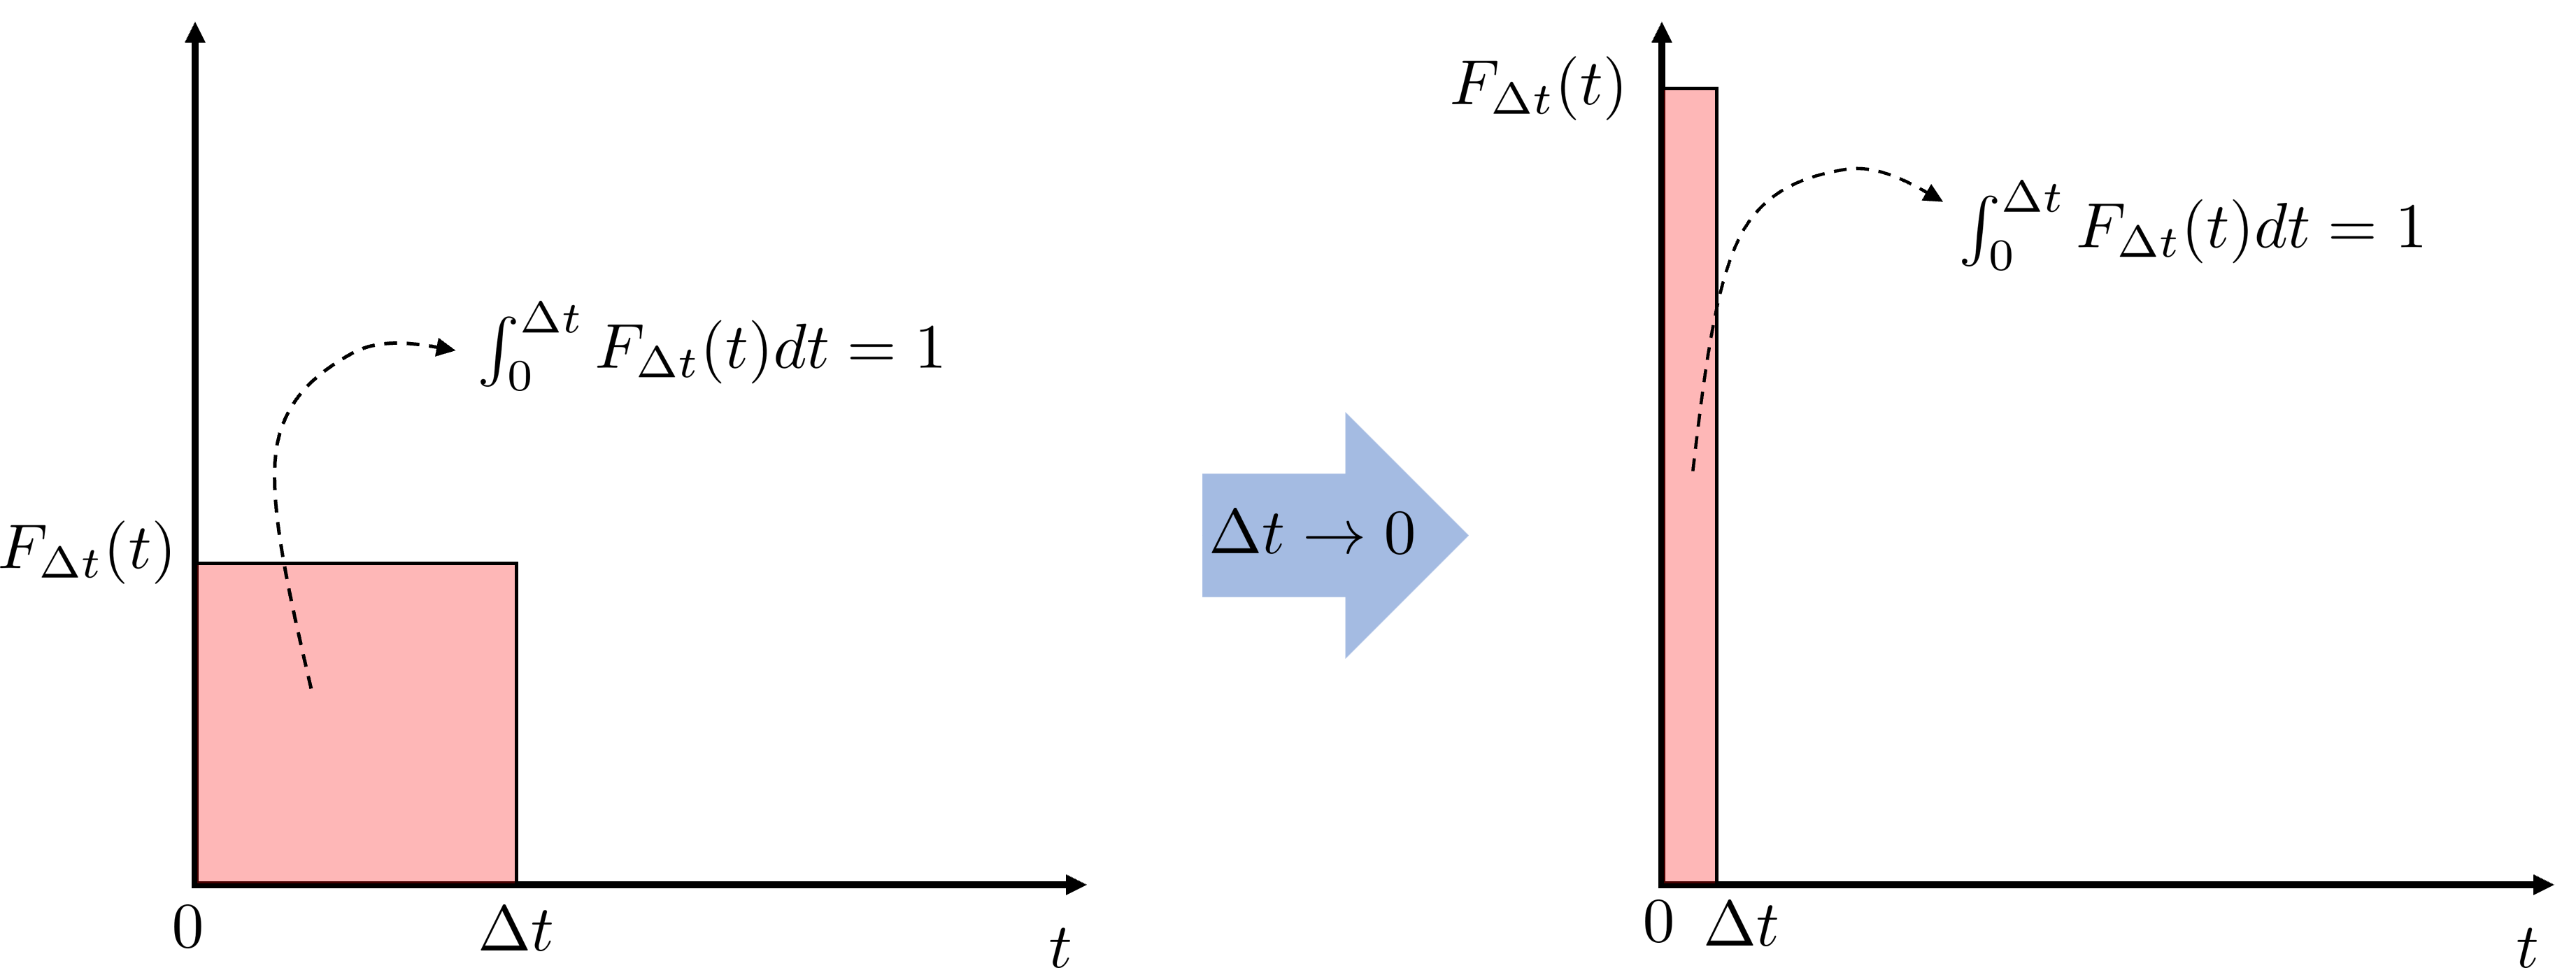
\includegraphics[width=20cm]{./FIG_Franklin/fig8-smc2.png}
	    \end{figure}

\end{enumerate}

   
    \newpage
    %!TEX root = ../main.tex
\setcounter{chapter}{7}
\setcounter{section}{0}
\section{Digitization}
\vspace{-8pt} \hrule \hrule \hrule \hrule \hrule  \vspace{12pt}

$\bigstar$ Unit step function
\begin{align*}
	1_k(t) = \frac{1}{1+e^{-2kt}}&&&& 1(t) = \begin{cases}1 & t \geq 0 \\0 & t< 0\end{cases}\\
	1(t) = \lim_{k \rightarrow \infty} 1_k(t) 
\end{align*}


	    \begin{figure}[!h]
	        \centering
	        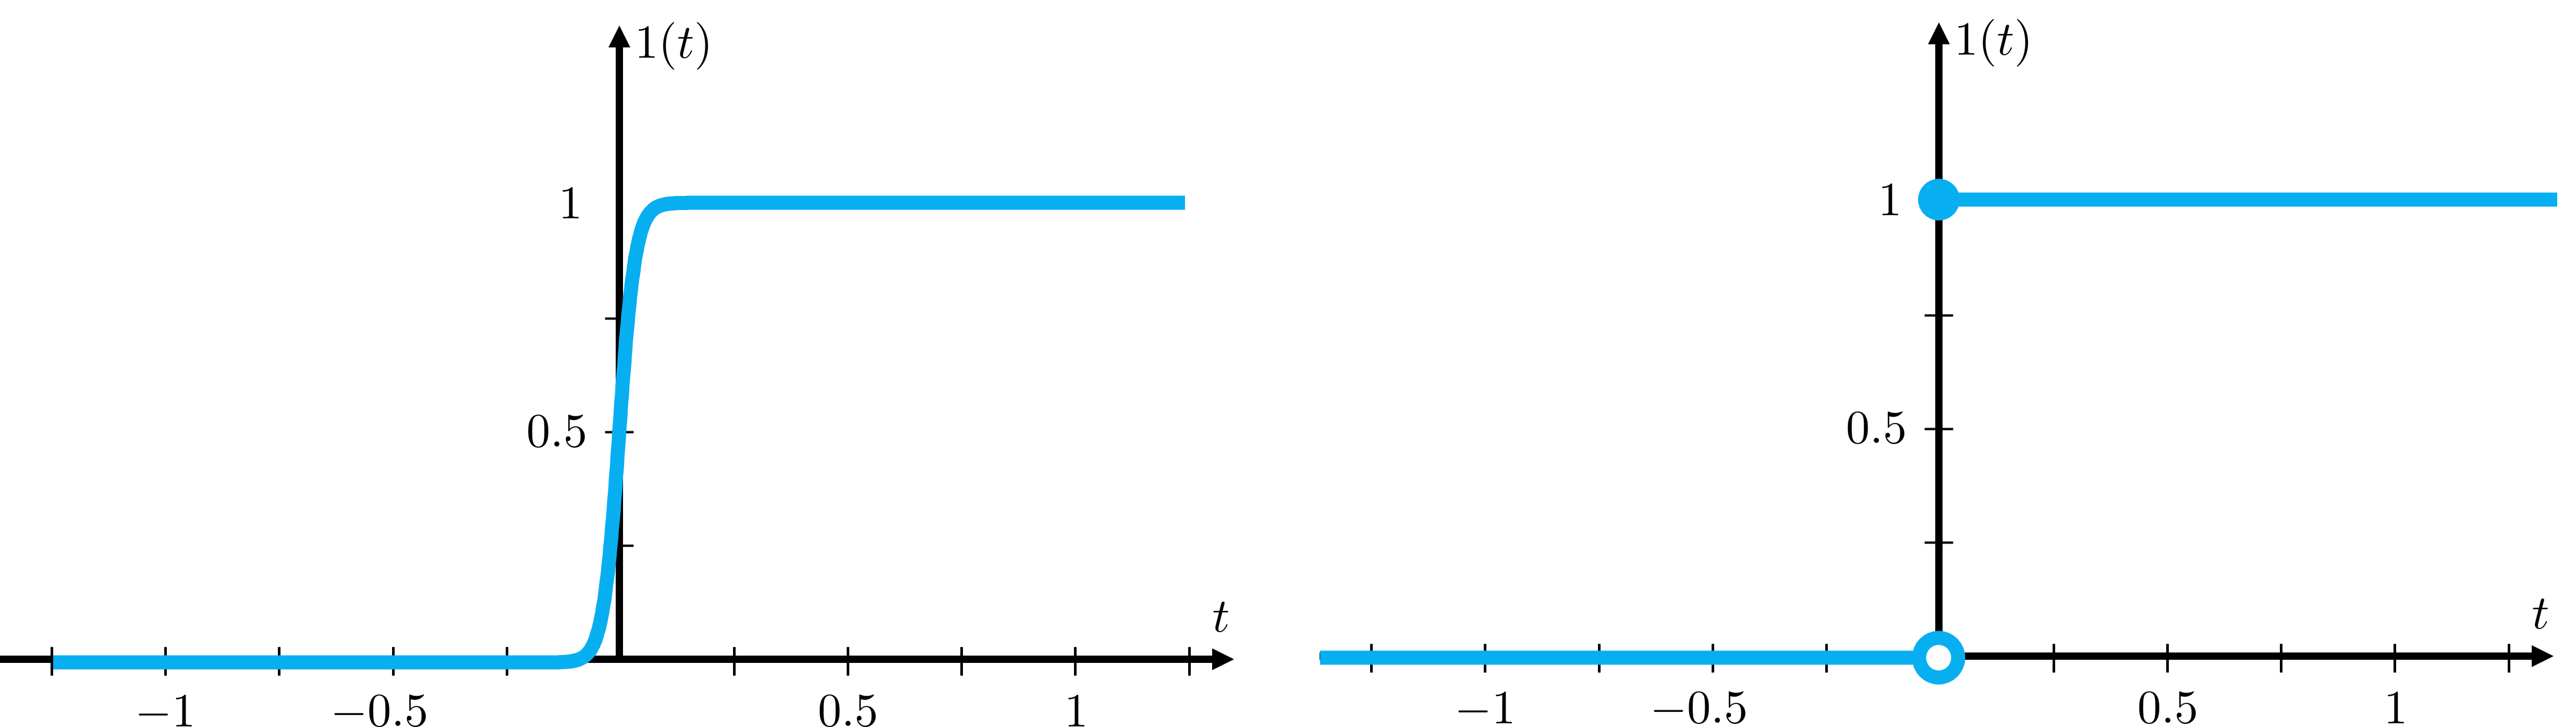
\includegraphics[width=18cm]{./FIG_Franklin/fig8-smc2_2.png}
	    \end{figure}


$\bigstar$ Useful Properties
 \begin{enumerate}
 	\item $\frac{d1(t)}{dt} = \delta(t) $ (수학적으로는 틀림, 개념적으로 사용)
 	\item $x(t)\delta(t-kT) = x(kT)\delta(t-kT)$
 	\item $\int_{-\infty}^{\infty} x(t) \delta(t-kT) dt= x(kT)$\\
		$ \because \int_{-\infty}^{\infty} x(t) \delta(t-kT)dt =\int_{-\infty}^{\infty} x(kT) \delta(t-kT) dt=x(kT)\int_{-\infty}^{\infty} \delta(t-kT) dt=x(kT)$
 	
 
 \end{enumerate}


   
    \newpage
    %!TEX root = ../main.tex
\setcounter{chapter}{7}
\setcounter{section}{0}
\section{Digitization}
\vspace{-8pt} \hrule \hrule \hrule \hrule \hrule  \vspace{12pt}

$\bigstar$ Sampling Process
	    \begin{figure}[!h]
	        \centering
	        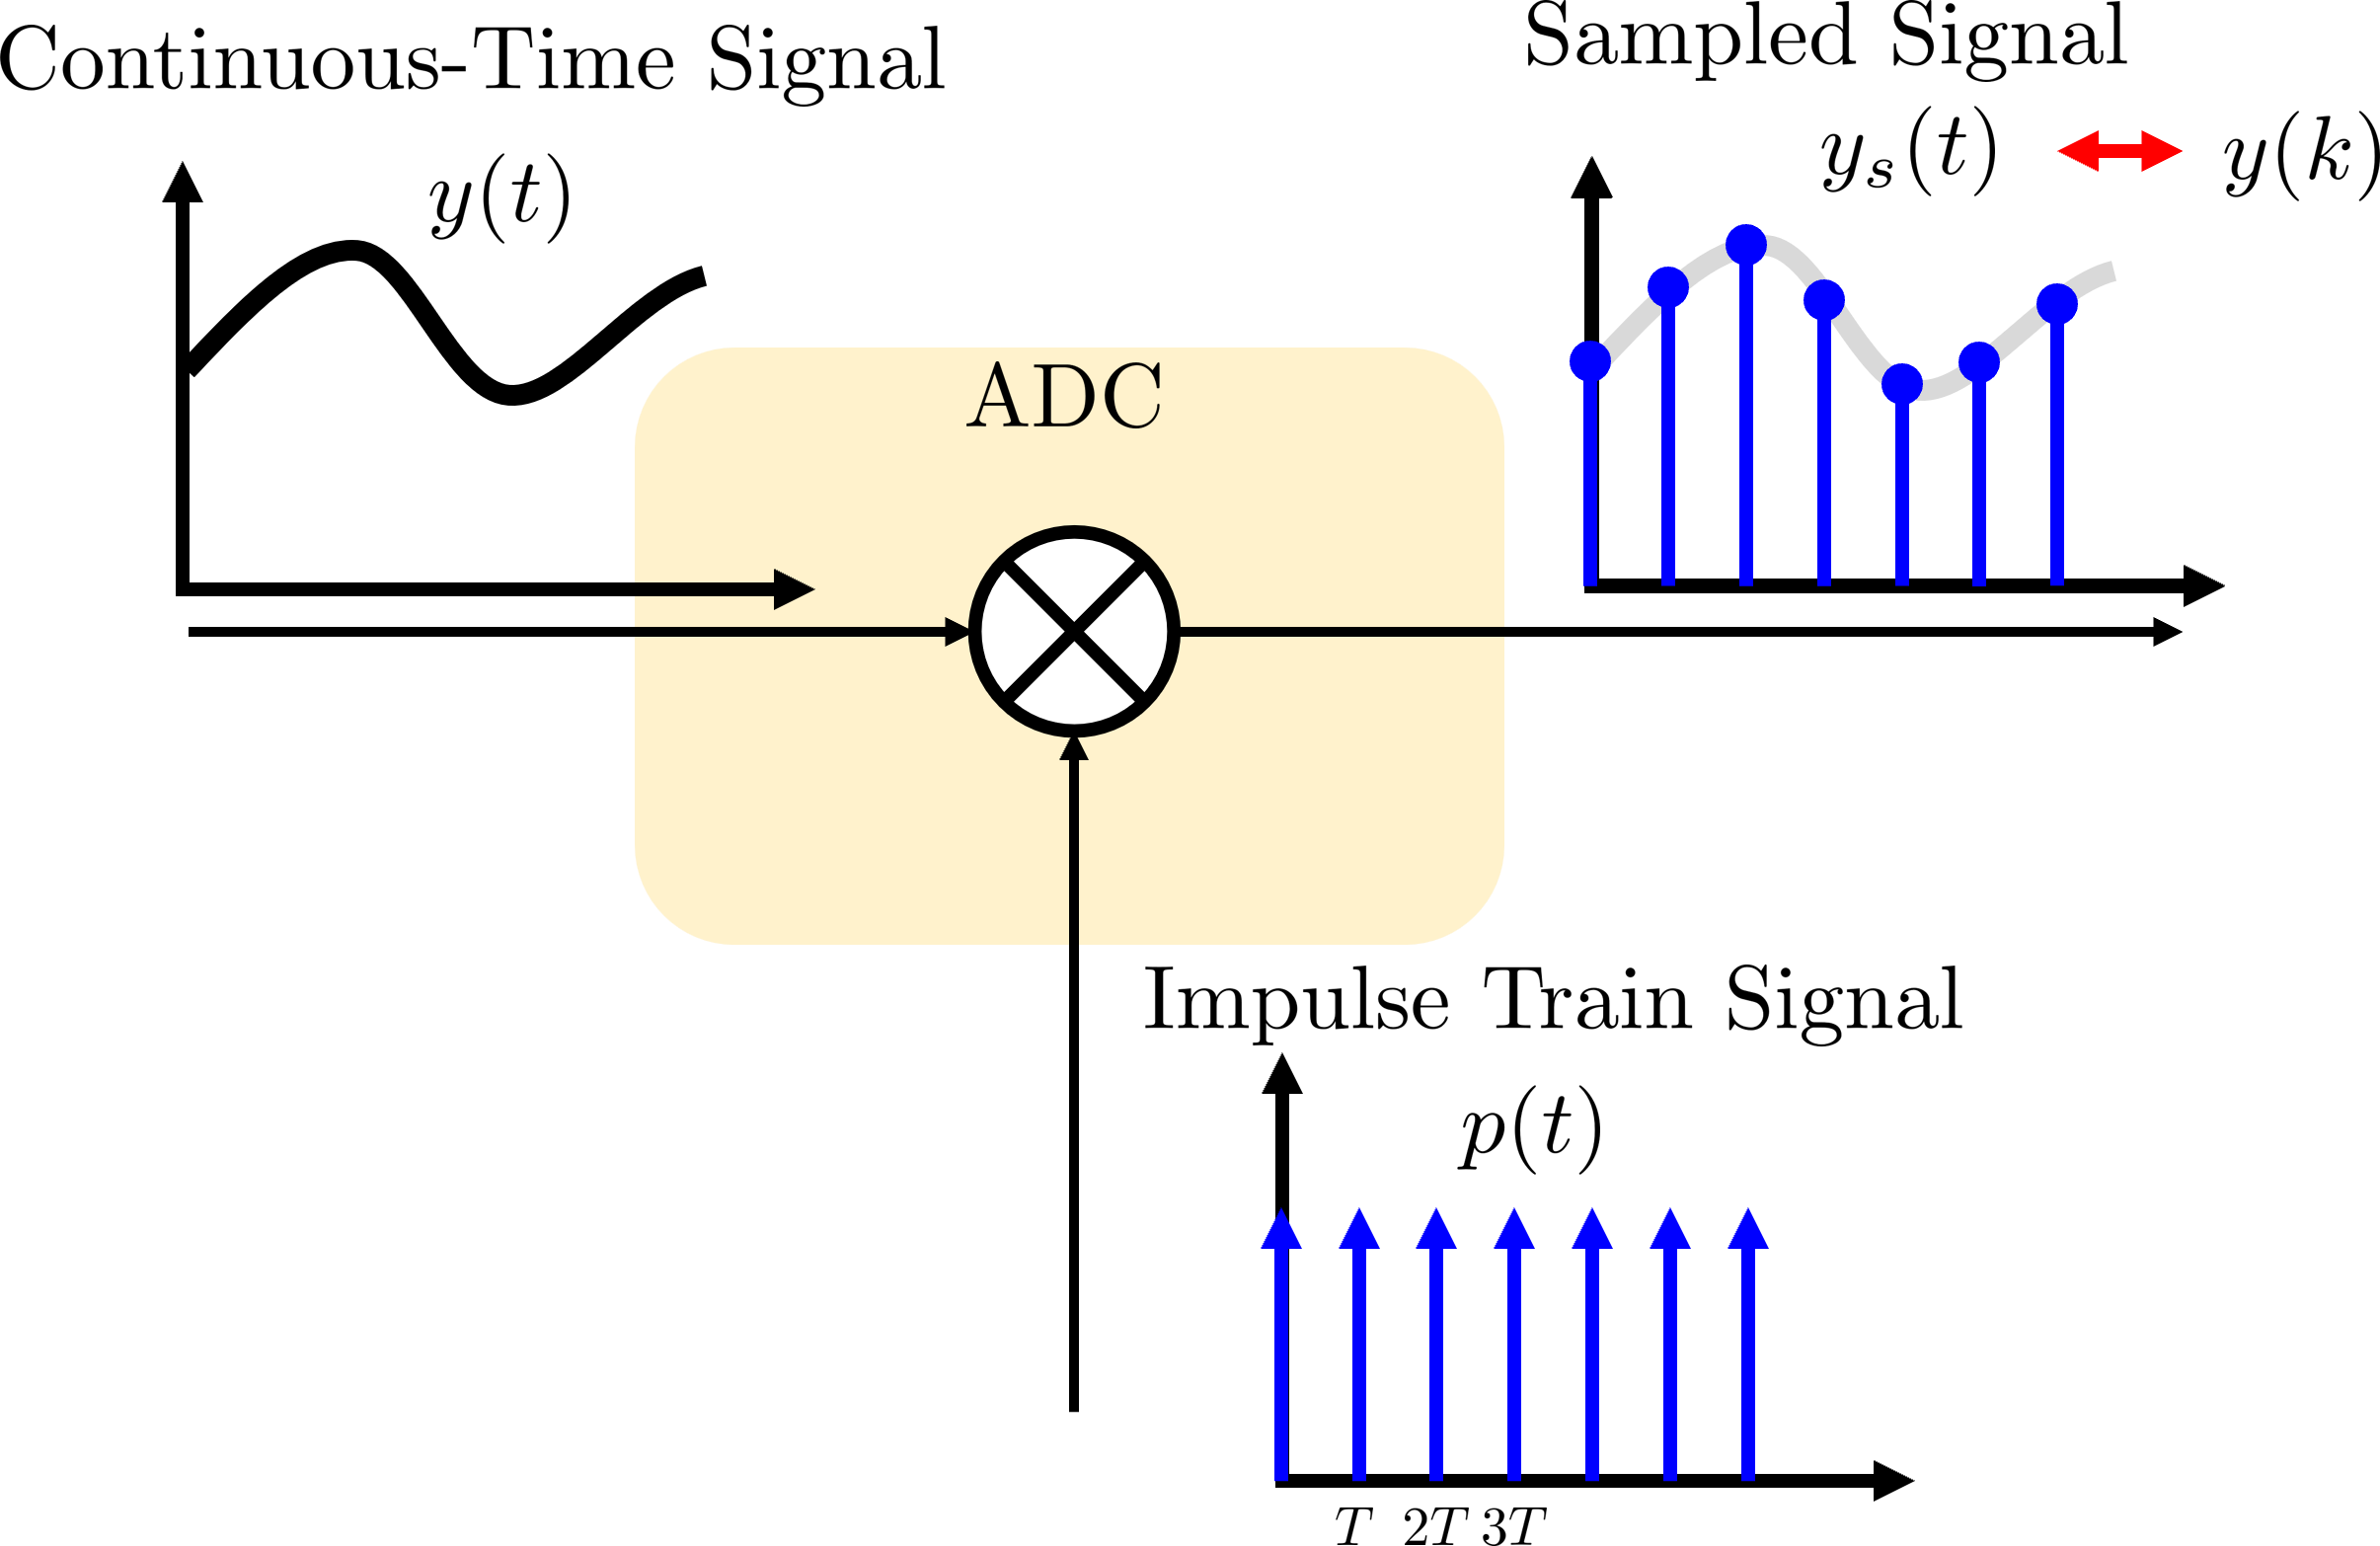
\includegraphics[width=10cm]{./FIG_Franklin/fig8-smc3.png}
	    \end{figure}
    \begin{enumerate}
    	\item Periodic Impulse Train: p(t) is periodic with period $T = 1/F_s$
    	\begin{align*}
    		p(t) = \sum_{k=-\infty}^{\infty} \delta(t-kT)
    	\end{align*}
     	\item Sampled Signal: we can consider $y_s(t)$ te be the analog equivalent to discrete-time signal $y(k)$ or $y(kT)$
    	\begin{align*}
    		y_s(t) &= y(t) \cdot p(t) = \sum_{k=-\infty}^{\infty} y(t)\delta(t-kT) = \sum_{k=-\infty}^{\infty} y(kT)\delta(t-kT)\\
    			&\leftrightarrow y(k) = y(kT)
    	\end{align*}
	\end{enumerate}   
    \newpage
    %!TEX root = ../main.tex
\setcounter{chapter}{7}
\setcounter{section}{0}
\section{Digitization}
\vspace{-8pt} \hrule \hrule \hrule \hrule \hrule  \vspace{12pt}
$\bigstar$ Nyquist–Shannon Sampling Theorem
\begin{enumerate}
	\item 간단하게, 아날로그 신호가 갖는 최대 주파수의 2배이상의 샘플링 주파수를 사용해야만 손실되는 정보없이 디지털 신호를 아날로그 신호로 복원할 수 있다.
	\item Nyquist freqeuncy(Folding Frequency): Sampling Frequency $F_s$의 절반 $F_{nyquist}=F_s/2$이며, 이는 신호의 최대 주파수 $F_{nyquist} \geq F_{max} $ 이어야 신호를 복원 할 수 있다. 
	\item Frequency Domain Analysis:
	\begin{align*}
	    \text{time-domain}& &&&&\text{frequency-domain}\\
		y_s(t) = y(t)\cdot p(t) & & \leftrightarrow & &Y_{s}(F) = &Y(F) \ast P(F) \\
		&&&&=& Y(F) \ast \frac{1}{T} \sum_{k =-\infty}^{\infty}\delta(F-kF_s)\\
		&&&&=& \frac{1}{T} \sum_{k =-\infty}^{\infty} Y(F-kF_{s})
	\end{align*}
\end{enumerate}

   
    \newpage
    %!TEX root = ../main.tex
\setcounter{chapter}{7}
\setcounter{section}{0}
\section{Digitization}
\vspace{-8pt} \hrule \hrule \hrule \hrule \hrule  \vspace{12pt}
	    \begin{figure}[!h]
	        \centering
	        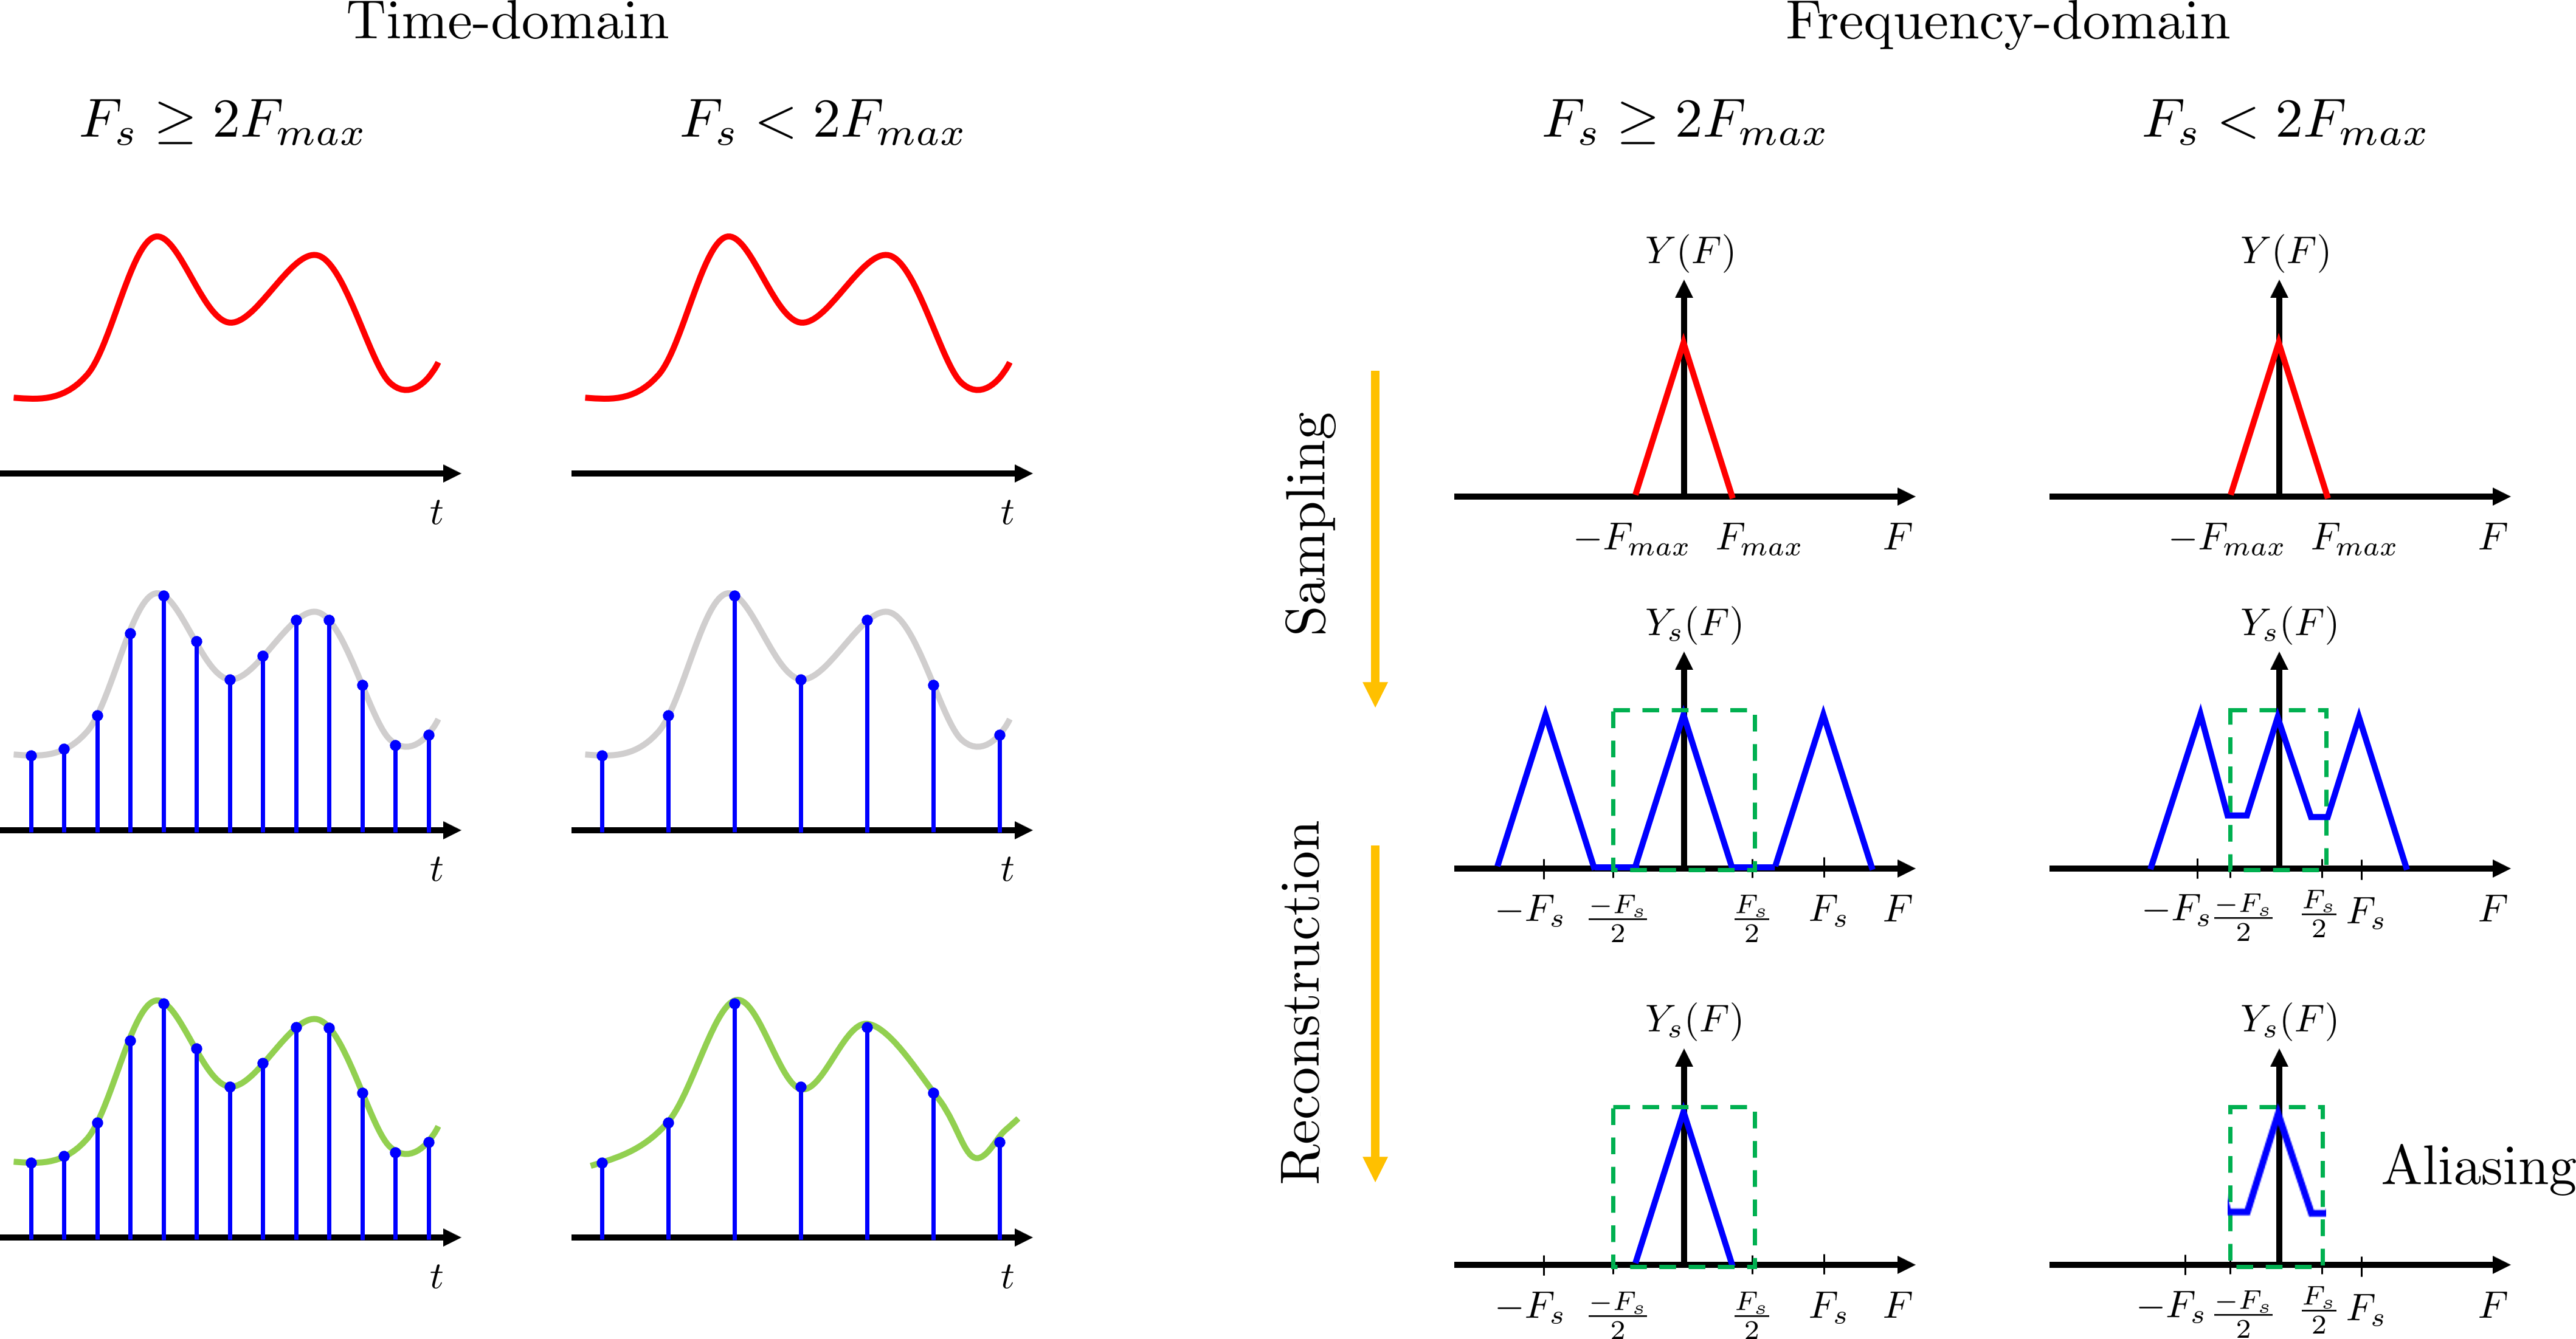
\includegraphics[width=24cm]{./FIG_Franklin/fig8-smc4.png}
	    \end{figure}   
    \newpage
    %!TEX root = ../main.tex
\setcounter{chapter}{7}
\setcounter{section}{0}
\section{Digitization}
\vspace{-8pt} \hrule \hrule \hrule \hrule \hrule  \vspace{12pt}

	    \begin{figure}[!h]
	        \centering
	        \includegraphics[width=24cm]{./FIG_Franklin/fig8-smc5.png}
	    \end{figure}
   
    \newpage    
    %!TEX root = ../main.tex
\setcounter{chapter}{7}
\setcounter{section}{1}
\section{Dynamic Analysis of Discrete Systems}
\vspace{-8pt} \hrule \hrule \hrule \hrule \hrule  \vspace{12pt}

% Please add the following required packages to your document preamble:
% \usepackage{booktabs}

\begin{table}[!hb]
\centering
\begin{tabular}{@{}|c|c|c|@{}}
\toprule
Condition                           & Discrete-Time                   & Continuous-Time   \\ \midrule
Periodic Signal                     & Discrete Fourier Series         & Fourier Series    \\ \midrule
Absolute Summable/Integrable Signal & Discrete-Time Fourier Transform & Fourier Transform \\ \midrule
Causal Signal                       & Unilateral $z$-Transfrom          & Unilateral Laplace Transform \\ \bottomrule
\end{tabular}
\end{table}
\begin{itemize}
	\item $z$-transform for discrete time systems $\leftrightarrow$ Laplace transform for continuous time systems. 
\item (8.2.1) $z$-Transform 
	\begin{enumerate}
		\item Laplace transform and its important property 
		\begin{align*}
			\mathcal{L} (f(t))&= F(s) = \int_{0^-}^{\infty} f(t) e^{-st} dt 
			&&&
			\mathcal{L}(\dot{f}(t)) &= sF(s) -f(0^{-})\\
			&&\Downarrow&
			\\
						\mathcal{L} (f(t))&= F(s) = \int_0^{\infty} f(t) e^{-st} dt 
			&&&
			\mathcal{L}(\dot{f}(t)) &= sF(s) \text{ } \text{ where $f(0^+) = 0$}
		\end{align*}
		$0^{-}$부터인 이유는 $f(t)$가 $\delta(t)$나 $\frac{d\delta(t)}{dt}$일때 Laplace Transform에 반영하기 위함, 이해를 돕기위해 정확한 정의는 아니지만 아래와 같은 정의 사용
	\end{enumerate}	
\end{itemize}

   
    \newpage    
    %!TEX root = ../main.tex
\setcounter{chapter}{7}
\setcounter{section}{0}
\section{Digitization}
\vspace{-8pt} \hrule \hrule \hrule \hrule \hrule  \vspace{12pt}

	\begin{enumerate}	
		\setcounter{enumi}{1}



	\item $z$-transform is defined by 
		\begin{align*}
			\mathcal{Z}(f(k)) &= F(z) = \sum_{k=0}^{\infty} f(k) z^{-k}  
			&&&
			\mathcal{Z} (f(k-1)) &=   \sum_{k=0}^{\infty} f(k-1) z^{-k}  
			\\
			&= f(0) + f(1) z^{-1} + f(2) z^{-2} + \cdots
			&&&
			&= f(-1) + f(0) z^{-1} + f(1) z^{-2} + f(2) z^{-3} + \cdots \\
			& &&& &= z^{-1} \left[  f(0) + f(1) z^{-1} + f(2) z^{-2} + \cdots \right] \\ 
			& &&& &= z^{-1} F(z) 
		\end{align*}
		where $f(k)$ is the sampled version of $f(t)$ and $z^{-1}$ represents one sample delay, and $f(-1) = 0$. \\

		Example) $x(0) = 0 ,x(1) = 1, x(2) = 2 ,x(3) = 3, x(4) = 4 $		\\
		\begin{flalign}
		 X(z) &= \sum_{k=0}^{\infty} x(k)z^{-k}\\
		      &=x(0) + x(1)z^{-1}+ x(2)z^{-2}+ x(3)z^{-3}+ x(4)z^{-4} \\
		      &= z^{-1}+2z^{-2}+3z^{-3}+4z^{-4}
        \end{flalign}
		\item Important property between LT and $z$-transform
		\begin{align*}
			z = e^{sT} ~~~~ \leftrightarrow~~~~ s = \frac{1}{T} \ln z  
		\end{align*}
		\item For example, the general second-order difference equation 
		\begin{align*}
			y(k) = -a_1 y(k-1) - a_2 y(k-2) + b_0 u(k) + b_1 u(k-1) + b_2 u(k-2) 
		\end{align*}
		can be converted from this form to the $z$-transform of the variables $y(k)$ and $u(k)$ by invoking above relations,
		\begin{align*}
			Y(z) = (-a_1 z^{-1} - a_2 z^{-2}) Y(z) + (b_0 + b_1 z^{-1} + b_2 z^{-2}) U(z) 
		\end{align*}
		now we have a discrete transfer function:
		\begin{align*}
			\frac{Y(z)}{U(z)} = \frac{b_0 + b_1 z^{-1} + b_2 z^{-2}}{1 + a_1 z^{-1} + a_2 z^{-2}} 
		\end{align*}
	\end{enumerate}	
   
    \newpage    
    %!TEX root = ../main.tex
\setcounter{chapter}{7}
\setcounter{section}{1}
\section{Dynamic Analysis of Discrete Systems}
\vspace{-8pt} \hrule \hrule \hrule \hrule \hrule  \vspace{12pt}

	\begin{enumerate}	
		\setcounter{enumi}{3}
		\item For example, the general second-order difference equation 
		\begin{align*}
			y(k) = -a_1 y(k-1) - a_2 y(k-2) + b_0 u(k) + b_1 u(k-1) + b_2 u(k-2) 
		\end{align*}
		can be converted from this form to the $z$-transform of the variables $y(k)$ and $u(k)$ by invoking above relations,
		\begin{align*}
			Y(z) &= -a_1 z^{-1} Y(z) -a_2 z^{-2} Y(z) + b_0 U(z) + b_1 z^{-1} U(z) + b_2 z^{-2} U(z)\\
			     &= (-a_1 z^{-1} - a_2 z^{-2}) Y(z) + (b_0 + b_1 z^{-1} + b_2 z^{-2}) U(z) 
		\end{align*}
		now we have a discrete transfer function:
		\begin{align*}
			Y(z) - (-a_1 z^{-1} - a_2 z^{-2}) Y(z) &= (b_0 + b_1 z^{-1} + b_2 z^{-2}) U(z) \\
			(1 +a_1 z^{-1} + a_2 z^{-2}) Y(z) &= (b_0 + b_1 z^{-1} + b_2 z^{-2}) U(z) \\
			\frac{Y(z)}{U(z)} = \frac{b_0 + b_1 z^{-1} + b_2 z^{-2}}{1 + a_1 z^{-1} + a_2 z^{-2}} 
		\end{align*}

	\end{enumerate}	   
    \newpage   
    %!TEX root = ../main.tex
\setcounter{chapter}{7}
\setcounter{section}{1}
\section{Dynamic Analysis of Discrete Systems}
\vspace{-8pt} \hrule \hrule \hrule \hrule \hrule  \vspace{12pt}

\begin{itemize}	

\item (8.2.1) $z$-Transform 
	\begin{enumerate}
		\item See the Table 8.1 for understanding between $z$-transform and LT
		\begin{table}[h]
		\centering
			\begin{tabular}{c||c||c|c} 
				\hline \hline 
				$F(s)$ & $f(kT)$ & $F(z)$ & \\ \hline
				- & $\delta(kT)$ & 1 & 1 \\
				- & $\delta(kT-k_0 T)$ & $z^{-k_0}$ & $z^{-k_0}$ \\
				$\frac{1}{s}$ & $1(kT)$ & $\frac{z}{z-1}$ & $\frac{1}{1-z^{-1}}$ \\
				$\frac{1}{s^2}$ & $kT$ & $\frac{Tz}{(z-1)^2}$ & $\frac{Tz^{-1}}{(1-z^{-1})^2} $ \\
				$\frac{1}{s+a}$ & $e^{-akT}$ & $\frac{z}{z-e^{-aT}}$ & $\frac{1}{1-e^{-aT}z^{-1}}$ \\
				$\frac{1}{s(s+a)}$ & $1-e^{-akT}$ & $\frac{z(1-e^{-aT})}{(z-1)(z-e^{-aT})}$ & $\frac{z^{-1}(1-e^{-aT})}{(1-z^{-1})(1-e^{-aT} z^{-1})}$ \\
				$\frac{a}{s^2+a^2}$ & $\sin a kT$ & $\frac{z \sin aT}{z^2-(2\cos aT)z +1}$ & $\frac{z^{-1}  \sin aT}{1-(2\cos aT)z^{-1} + z^{-2}}$ \\
				$\frac{s}{s^2+a^2}$ & $\cos a kT$ & $\frac{z(z- \cos aT)}{z^2-(2\cos aT)z +1}$ & $\frac{(1- z^{-1}\cos aT )}{1-(2\cos aT)z^{-1} +z^{-2}}$ \\
				\hline \hline 
			\end{tabular}
		\end{table}
		\item For parts of Table, we have
		\begin{align*}
			\mathcal{Z}(\delta(kT)) &=\sum_{k=0}^{k=\infty}\delta(kT)z^{-k}= \delta(0 \cdot T) + \delta(1 \cdot T)z^{-1} + \cdots  = 1  + 0 z^{-1} + 0 z^{-2} + \cdots = 1  \\  
			\mathcal{Z}(\delta(k-k_0T)) &= 0  + 0 z^{-1} +  \cdots + 1 z^{-k_0} + \cdots +  = z^{-k_0}  \\  
			\mathcal{Z}(1(kT)) &= 1 + z^{-1} + z^{-2} + \cdots = \frac{1}{1-z^{-1}} = (1-z^{-1})^{-1}  \\
			\mathcal{Z}(e^{-akT}) &= 1 + e^{-aT} z^{-1} + e^{-2aT} z^{-2} + \cdots = \frac{1}{1-e^{-aT}z^{-1}} \\
		\end{align*}
	\end{enumerate}

\end{itemize}			   
    \newpage    
\end{document}
